\documentclass{beamer}
\usepackage[utf8]{inputenc} 
\title{Sergio Ramos}
\author{Patryk Sobolewski}
\institute{UWM}
\date{\today}
\usepackage{amsfonts}
\usepackage[MeX]{polski}
\usepackage{graphicx}
\begin{document}
\frame{\titlepage}



\begin{frame}
\frametitle{Spis Treści}
\tableofcontents
\end{frame}



\section{Życiorys}
\begin{frame}{}
\begin{itemize}
\item{Sergio Ramos García ;(ur. 30 marca 1986 w Camas) – hiszpański piłkarz występujący na pozycji obrońcy w hiszpańskim klubie Real Madryt, którego jest kapitanem. Reprezentant Hiszpanii.}
\begin{figure}
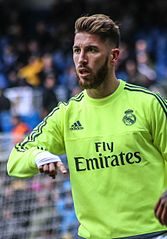
\includegraphics[width=0.25\hsize] {Sergio.jpg}
\caption{Sergio Ramos}\label{fig:Sergio}
\end{figure}
\end{itemize}
\end{frame}

\begin{frame}{Życiorys, cd.}
\begin{itemize}
\item<1>Karierę rozpoczynał w Sevilli. W sezonie 2004/2005 rozegrał 31 ligowych spotkań, udało mu się strzelić 2 bramki. Ramos był ostrzegany przez sędziów kartkami zaledwie pięciokrotnie. To niedużo, jak na środkowego obrońcę. 
\item<2>Świetne występy w Pucharze UEFA sprawiły, że okrzyknięto go najlepszym młodym graczem tych rozgrywek w sezonie 2004/2005. Ramos zaliczył także występy w młodzieżowej reprezentacji Hiszpanii do lat 21. Zadebiutował w niej w 2004 roku. Rozegrał 6 spotkań.
\item<3>Latem 2005 roku Real Madryt rozpoczął starania o przeprowadzenie transferu obrońcy Sevilli. Negocjacje zakończyły się sukcesem dopiero wieczorem 31 sierpnia, na chwilę przed zamknięciem okienka transferowego. Kwota transferu wyniosła 27 mln euro.
\end{itemize}
\end{frame}


\section{Kariera w reprezentacji}
\begin{frame}{Reprezentacja:}
\begin{itemize}

\item<1>W 2005 roku, mając 19 lat, utalentowany defensor, zadebiutował w pierwszej reprezentacji Hiszpanii. W ten sposób został najmłodszym graczem, który zadebiutował w drużynie z Półwyspu Iberyjskiego od 55 lat. Następstwem dobrej gry były występy w trudniejszych i ważniejszych meczach, podczas eliminacji do Mistrzostw Świata.
\item<2>Hiszpania grała mecz o wszystko z Serbią. Podczas nieobecności Míchela Salgado, swoje umiejętności mógł zaprezentować Ramos. Mimo młodego wieku zdołał upilnować tak renomowanych piłkarzy jak Mateja Kežman, Savo Milošević czy Dejan Stanković.
\end{itemize}
\end{frame}

\begin{frame}{Ważne momenty życiowe:}
\begin{itemize}
\item{Selekcjoner reprezentacji Hiszpanii Luis Aragonés postanowił zabrać go na Mistrzostwa Świata w Piłce Nożnej 2006 do Niemiec, gdzie pomógł drużynie dotrzeć do 1/8 finałów.
\begin{figure}
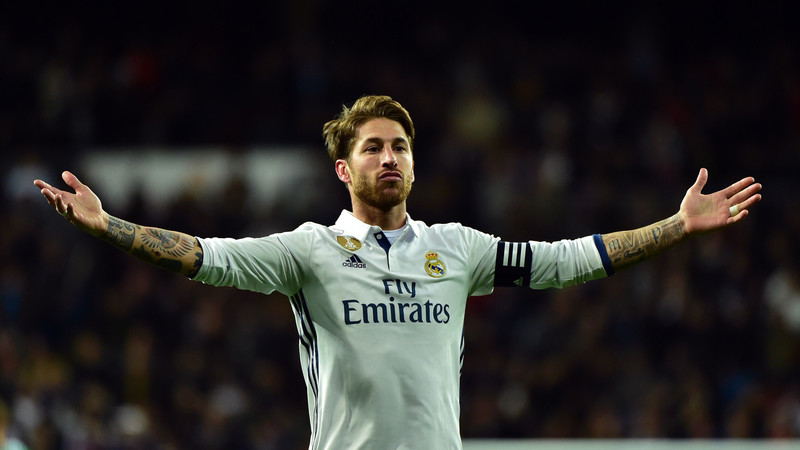
\includegraphics[width=0.5\hsize] {ss.jpg}
\label{fig:ss}
\end{figure}
}
\end{itemize}
\end{frame}


\begin{frame}{Statystyki kariery:}
\begin{itemize}
\section{Statystyki kariery}

\begin{table}
\begin{tabular}{lcr}
\hline
\textbf{Sezon}&\textbf{Mecze}&\textbf{Gole}&\textbf{Asysty}\\
\hline
2003{/}04&7&0&0\\
2004{/}05&31&2&0\\
2005{/}06&33&4&0\\
2006{/}07&33&5&2\\
2007{/}08&33&5&4\\
2008{/}09&32&4&3\\
2009{/}10&33&4&5\\
20010{/}11&31&3&2\\
20011{/}12&34&3&6\\
20012{/}13&26&4&0\\
20013{/}14&32&4&1\\
20014{/}15&27&4&1\\
20015{/}16&23&2&3\\
\hline
\end{tabular}
\end{table}

\end{itemize}
\end{frame}


\section{Sukcesy}
\begin{frame}{Real Madryt}
\begin{itemize}
\item Klubowe mistrzostwo świata: 2014, 2016
\item Superpuchar Europy UEFA: 2014, 2016, 2017
\item Liga Mistrzów UEFA: 2013/2014, 2015/2016, 2016/2017
\item Mistrzostwo Hiszpanii: 2006/2007, 2007/2008, 2011/2012, 2016/2017
\item Puchar Hiszpanii: 2010/2011, 2013/2014
\item Superpuchar Hiszpanii: 2008, 2012, 2017
\end{itemize}
\end{frame}

\begin{frame}{Reprezentacja}
\begin{itemize}
\item Mistrzostwo Europy U-19 2004  Złoto
\item Mistrzostwo Europy 2008  Złoto
\item Puchar Konfederacji: 2009 Brąz
\item Mistrzostwo Świata 2010 Złoto
\item Mistrzostwo Europy 2012 Złoto
\item Puchar Konfederacji: 2013 Srebro
\end{itemize}
\end{frame}

\begin{frame}{Indywidualne}
\begin{itemize}
\item Najlepszy zawodnik La Liga poniżej 20. roku życia według UEFA: 2005
\item Najlepszy obrońca na świecie poniżej 20. roku życia według UEFA: 2006
\item Don Balón Award: 2005
\item Jedenastka Roku według ESM: 2008, 2012
\item FIFPro World XI: 2008, 2011, 2012, 2013, 2014
\item Drużyna Roku UEFA: 2008, 2012, 2013, 2014
\item Antonio Puerta Award: 2008
\item Móstoles Sports Elite Award: 2009
\item Najlepszy zawodnik Mistrzostw Świata 2010 w RPA według Castrol Index
\item Jedenastka marzeń według FIFA podczas Mistrzostw Świata 2010 w RPA
\item Najlepszy zawodnik Mistrzostw Europy 2012 w Polsce i Ukrainie według Castrol Index
\item Drużyna marzeń według UEFA podczas Mistrzostw Europy 2012 w Polsce i Ukrainie
\item Najlepszy obrońca Primera División: 2012, 2013, 2014
\item Najlepszy zawodnik Klubowych Mistrzostw Świata: 2014
\item Drużyna sezonu Ligi Mistrzów: 2016/2017
\end{itemize}
\end{frame}

\section{Życie prywatne}
\begin{frame}{Prywatnie:}
\begin{itemize}
Piłkarz jest w związku z Pilar Rubio, hiszpańską reporterką. 6 maja 2014 na świat przyszedł Sergio Ramos Rubio, pierwsze dziecko pary. Agentem Sergia Ramosa jest jego brat, Rene.


\end{itemize}
\end{frame}

\end{document}
